%%
% The BIThesis Template for Bachelor Paper Translation
%
% 北京理工大学毕业设计(论文) —— 使用 XeLaTeX 编译
%
% Copyright 2020-2023 BITNP
%
% This work may be distributed and/or modified under the
% conditions of the LaTeX Project Public License, either version 1.3
% of this license or (at your option) any later version.
% The latest version of this license is in
%   http://www.latex-project.org/lppl.txt
% and version 1.3 or later is part of all distributions of LaTeX
% version 2005/12/01 or later.
%
% This work has the LPPL maintenance status `maintained'.
%
% The Current Maintainer of this work is Feng Kaiyu.
%
% Compile with: xelatex -> biber -> xelatex -> xelatex
%%

% 第一章节

\chapter{外文原文}

\section{Quick Start}

All of the Substrate tutorials and how-to guides require you to build and run a Substrate node in your development environment.
To help you set up a working environment quickly, the Substrate Developer Hub (https://github.com/substrate-developer-hub/) maintains several _templates_ for you to use.
For example, the Developer Hub substrate-node-template (https://github.com/substrate-developer-hub/substrate-node-template/tags/) is a snapshot of the main Substrate node-template binary that includes everything you need to get started with a functional node and a core set of features.

This _Quick start_ assumes that you are setting up a development environment for the first time and want to try out running a single blockchain node on your local computer.
To keep things simple, you'll connect to the local node using a web browser and look up a balance for a predefined sample account.

\subsection{Before you begin}


Before you begin, verify the following: 

\begin{itemize}
  \item You have an internet connection and access to an interactive shell terminal on your local computer.
  \item You are generally familiar with software development and using command-line interfaces.
  \item You have the Rust compiler and toolchain installed.
  You can check whether you have Rust installed by running the rustup show command.
\end{itemize}

If Rust is installed, this command displays version information for the toolchain and compiler.
If Rust is not installed, the command doesn't return any output.
For information about installing Rust, see [Install] (/install).

\subsection{构建节点模板}

\begin{enumerate}
  \item 将节点模板的仓库通过下列指令克隆到本地:
        \begin{lstlisting}
  git clone https://github.com/substrate-developer-hub/substrate-node-template
  \end{lstlisting}

        在绝大多数情况下,您只需克隆`main`分支即可获得最新的代码。不过,您也可以使用`--branch`选项选择特定分支以搭配特定版本的Polkadot使用。关于不同分支和不同版本的Polkadot的适配情况,请参阅\href{https://github.com/substrate-developer-hub/substrate-node-template/tags}{Tags}。

  \item 在终端中,切换工作目录到克隆下来的仓库文件夹中:
        \begin{lstlisting}
    cd substrate-node-template
  \end{lstlisting}
        若您想让自己的分支更有辨识度,或是更易于保存属于您自己的修改,您可以使用形如下列指令来创建一个新的分支:
        \begin{lstlisting}
          git switch -c my-branch-v0.9.29
        \end{lstlisting}
  \item 编译节点模板:
        \begin{lstlisting}
    cargo build --package node-template --release
  \end{lstlisting}
        由于所用的软件包数量较多,编译可能花费长达数分钟才能完成。
\end{enumerate}

\subsection{启动节点}

\begin{enumerate}
  \item 运行下列指令,确认您的节点已经就绪,并查看可用的命令行选项:
        \begin{lstlisting}
    ./target/release/node-template --help
  \end{lstlisting}

        通过上述命令获得的信息,我们可以知晓用于下列目的的命令行选项:
        \begin{itemize}
          \item 启动节点
          \item 处理账户
          \item 修改节点操作
        \end{itemize}

  \item 运行下列指令,查看预定义的开发账号`Alice`的信息:
        \begin{lstlisting}
    ./target/release/node-template key inspect //Alice
  \end{lstlisting}
        该指令将显示如下信息:
        \begin{lstlisting}
          Secret Key URI `//Alice` is account:
        Network ID:        substrate
        Secret seed:       0xe5be9a5092b81bca64be81d212e7f2f9eba183bb7a90954f7b76361f6edb5c0a
        Public key (hex):  0xd43593c715fdd31c61141abd04a99fd6822c8558854ccde39a5684e7a56da27d
        Account ID:        0xd43593c715fdd31c61141abd04a99fd6822c8558854ccde39a5684e7a56da27d
        Public key (SS58): 5GrwvaEF5zXb26Fz9rcQpDWS57CtERHpNehXCPcNoHGKutQY
        SS58 Address:      5GrwvaEF5zXb26Fz9rcQpDWS57CtERHpNehXCPcNoHGKutQY
        \end{lstlisting}

  \item 通过下列指令,您可以以开发模式启动节点:
        \begin{lstlisting}
    ./target/release/node-template --dev
  \end{lstlisting}

        在该模式下,该区块链不需要任何对等计算机以封装区块。节点启动后,终端将显示其所执行的操作的输出信息。若您看到形如“区块正在被提交/封装”,则说明您的节点已经开始正常运行:
        \begin{lstlisting}
    ... Idle (0 peers), best: #3 (0xcc78…5cb1), finalized #1 ...
    ... Starting consensus session on top of parent ...
    ... Prepared block for proposing at 4 (0 ms) ...
  \end{lstlisting}
\end{enumerate}

\subsection{连接到节点}

\begin{enumerate}
  \item 创建一个内含JavaScript以及\href{https://polkadot.js.org/docs/}{Polkadot-JS API}的HTML文件,以和节点互动。
  在本例中,我们将创建一个名为`index.html`的文件,其内含的JavaScript以及HTML代码将可以:
        \begin{itemize}
          \item 选择一个账号作为输入
          \item 使用onClick事件来查阅账号信息
          \item 作为以上两步骤的输出,显示该账号的余额信息
        \end{itemize}

        这份\href{https://docs.substrate.io/assets/quickstart/}{示例index.html}提供了使用JS、Polkadot-JS
        API和HTML进行以上步骤的简单演示。
  \item 复制粘贴\href{https://github.com/substrate-developer-hub/substrate-docs/blob/main/static/assets/quickstart/index.html}{上述示例HTML文件的源代码}至您的代码编辑器中,并保存为index.html至本地。
  \item 在浏览器中打开index.html。
  \item 复制账号Alice的SS58地址到网页中的输入框中,然后点击Get Balance按钮。
\end{enumerate}

\subsection{关闭节点}
\begin{enumerate}
  \item 找到之前显示区块链操作信息的终端。
  \item 键盘输入Ctrl + C以终止节点工作。
\end{enumerate}

\subsection{下一步做什么?}

在本节快速开始指南中,您学习了在本地计算机上编译并运行一个单链区块链的方法。若想学习各种功能的个性化设置,请参阅以下资源:

\begin{itemize}
  \item \href{https://docs.substrate.io/fundamentals/architecture/}{架构}
  \item \href{https://docs.substrate.io/fundamentals/runtime-development/}{运行时开发}
  \item \href{https://docs.substrate.io/fundamentals/rust-basics/}{为Substrate服务的Rust}
\end{itemize}

\section{基础知识}

基础知识章节的话题将围绕Substrate开发环境的核心准则和独特功能特性展开;此外,我们也将强调数个可供区块链开发者选择的设计选项。

Substrate提供了一组模块化的、灵活的工具库,为您在开发不同特定用途的区块链时随意选择、组合、修改并复用。无论是在私有网络中运行,抑或是经由Polkadot与其他区块链联动,Substrate均能胜任。

本章的话题将帮助您了解:通过Substrate能够搭建起什么样的区块链系统?这些系统能够贴合您的实际需求的秘诀又何在?


在我们正式使用Substrate开始开发之前,请您了解以下板块的知识:

\begin{itemize}
\item
  \href{/fundamentals/blockchain-basics/}{区块链基础}
  向您解释了开发区块链系统的复杂程度,并介绍了常见的区块链概念、组件和术语。
\item
  \href{/fundamentals/why-substrate/}{为何选择Substrate?}
  强调了Substrate所提供的,其他大部分区块链与智能合约平台所不具有的关键优点。
\item
  \href{/fundamentals/what-is-substrate/}{Substrate是什么?}
  解释了Substrate设计背后的核心理念,以及设计决策对我们使用的技术的影响。
\item
  \href{/fundamentals/architecture/}{架构}
  描绘了Substrate中节点架构的关键组件,以及这些组件如何与您自己的个性化区块链设计架构相关联。
\item
  \href{/fundamentals/node-and-network-types/}{网络与区块链}
  定义了在不同区块链部署场景下的不同拓扑结构,以及它们在基于Substrate的区块链中的实现。
\item
  \href{/fundamentals/runtime-development/}{运行时开发}
  强调了Substrate运行时的重要性,介绍了Substrate运行时的核心应用接口和运行之的最低要求。
\item
  \href{/fundamentals/consensus/}{共识}
  介绍最常见的共识模型,以及您能够在Substrate区块链上使用的共识模型的种类。
\item
  \href{/fundamentals/transaction-types/}{交易与区块基础}
  介绍交易的种类,以及构成一个区块的组件。
\item
  \href{/fundamentals/transaction-lifecycle/}{交易周期}
  介绍交易是如何被接收、排队处理,并最终封装进区块的。
\item
  \href{/fundamentals/state-transitions-and-storage/}{状态转换与存储}
  描述在运行时中,状态如何转换与存储,以及使用字典树和键值对加以管理。
\item
  \href{/fundamentals/accounts-addresses-keys/}{账户、地址与密钥}
  介绍了账户、地址与密钥的相互关系以及它们的用途。
\item
  \href{/fundamentals/rust-basics/}{为Substrate所用的Rust}
  强调了Rust特有的traits(特征)、泛型,关联类型和宏。熟练掌握这些知识,您就能顺利地构建基于Substrate的区块链了。
\item
  \href{/fundamentals/offchain-operations/}{离链操作}
  揭示了一部分操作最好离链操作的原因,以及它们的平替。
\item
  \href{/fundamentals/light-clients-in-substrate-connect/}{Substrate连接中的轻量级客户端}
  介绍了使用Substrate连接在您的应用程序中嵌入一个轻量级客户端的方法,以与其他基于Substrate的链互交互。
\item
  \href{/fundamentals/xcm-communication/}{跨共识通信}
  一份有关跨共识通信及其通信格式的概述。
\end{itemize}

在您消化了以上章节的知识之后,您就已经完全准备好设计、构建、测试属于您的区块链了。

\subsection{区块链基础}

区块链是一个去中心化的分布式账本,它以一系列的区块记录信息。区块包含的信息是一组有序的指令集合,这些指令可能导致状态的变化。

在区块链网络中,各个计算机(称为节点)相互通信,形成了去中心化的点对点(P2P)网络。在这样的网络中,并不存在所谓中央权威机构控制;每个参与区块生成的节点,都存储着组成所有节点公认的区块链区块的副本。

多数情况下,用户通过提交请求来与区块链交互,这些请求可能导致区块链的状态转变。例如,一个请求可能改变一份文件的所有权,或者在两个账户之间转移资产。这些交易请求将由网络中的其他节点传播,并由区块生产者(block
author)封装成一个区块。

为了确保链上数据的安全性和链上正在进行的事务的进度,节点使用某种形式的共识,就每个区块中的数据状态和已完成执行的事务的顺序达成一致。

\hypertarget{ux4ec0ux4e48ux662fux533aux5757ux94feux8282ux70b9}{%
\subsubsection{什么是区块链节点?}\label{ux4ec0ux4e48ux662fux533aux5757ux94feux8282ux70b9}}

抽象至一定高度后,所有的区块链节点都可以认为由以下四部分组成:

\begin{itemize}
\item
  数据存储区,它们记录交易之后产生的不同状态
\item
  点对点网络,用于去中心化地与其他节点通信
\item
  共识算法,用于保护自己免受恶意攻击者的攻击,确保链上事务顺利执行
\item
  为收到的交易进行排序、处理的算法逻辑
\item
  加密算法,用于为区块生成哈希摘要,为交易进行签名,以及验证收到的交易的签名
\end{itemize}

由于搭建区块链系统所需的核心组件的实现复杂度非常大,大多数区块链项目都是基于一份现成的代码作为基础,这样一来,程序员就可以通过修改已有代码来增添新功能,而非自己从零实现一个了。

例如,Litecoin、ZCash、Namecoin和Bitcoin
Cash都是从比特币的代码仓库中fork出去的。相似地,Quorom,POA
Network,KodakCoin和Musicoin是从以太坊的代码仓库fork出去的。

然而,大多数区块链平台并不是为个性化定制区块链而准备的。其结果就是,仅仅通过fork已有的仓库来构建新区块链有非常严重的局限性,包括但不限于原区块链代码带来的可延展性差等问题。

在我们探索Substrate在区块链项目中缓解上述问题的妙招之前,您很有必要了解一些大部分区块链共有的常见属性。通过学习大部分区块链的操作方法,您将更好地了解Substrate如何为构建最适合您需求的区块链提供替代方案和功能。

\hypertarget{ux72b6ux6001ux8f6cux6362ux4e0eux51b2ux7a81}{%
\subsubsection{状态转换与冲突}\label{ux72b6ux6001ux8f6cux6362ux4e0eux51b2ux7a81}}

区块链的本质是\href{(https://en.wikipedia.org/wiki/Finite-state_machine)}{状态机}。

在状态机运行的任意时刻,它都拥有一个内部的状态。

当执行收到的交易时,它们会导致状态的更改,因此区块链必须从当前状态转换到新状态。

但是,可能存在多个有效转换,这些转换将导致不同的新状态,区块链必须在其中选择一个,使之可以与其他节点产生共识。

为了就状态转换之后的新状态达成共识,所有区块链中的操作都必须是确定的。为使链能够正常运转,居多数的节点必须就状态转换之后的新状态达成共识,这包括:

\begin{itemize}
\item
  这条链的初始状态,又被称作``创世状态''或者``创世区块''
\item
  每一块区块中记录的,因发生交易而产生的状态变化
\item
  链中即将加入的,最终的状态
\end{itemize}

在中心化的网络中,``中心权威机构''可以在互斥状态转换之间进行选择。例如,配置为主要授权机构的服务器可能会按照看到它们的顺序,记录状态转换的更改;或者在冲突发生时,使用加权的算法在相互冲突的方案之间进行选择。

区块链用于将事务批量处理成区块并选择哪个节点可以向链提交区块的方法,称为区块链的共识模型或共识算法。最常用的共识模型被称为工作量证明共识模型。在工作量证明共识模型中,第一个完成计算问题的节点才有权向链提交区块。

为了使区块链具有容错能力并令所有节点拥有一致的状态,一些共识模型要求:即使某些节点受到恶意行为者干扰或网络中断威胁,至少三分之二的节点也必须在任何时候都对状态达成一致。

这三分之二的多数节点确保了网络是容错的,并且可以承受一些网络参与者的不良行为,无论这些行为是故意的还是偶然的。

\hypertarget{ux533aux5757ux94feux7ecfux6d4e}{%
\subsubsection{区块链经济}\label{ux533aux5757ux94feux7ecfux6d4e}}

所有区块链都需要资源来执行各种操作,例如处理器、内存、存储和网络带宽。参与网络的计算机(生产区块的节点)会向区块链用户提供这些资源。这些节点创建了一个分布式的、去中心化的网络,以满足网络用户(社区)的需求。

为了维护社区运转并使区块链可持续发展,大多数区块链要求用户以手续费的形式为他们使用的网络资源付费。要支付手续费,用户的身份就必须与持有某种类型资产的账户相关联。区块链通常使用``代币''来代表账户中的资产价值,用户通过``交易所''在链外购买代币。这样一来,用户就可以获得代币,为他们的交易付款了。

\hypertarget{ux533aux5757ux94feux7ba1ux7406ux65b9ux6cd5}{%
\subsubsection{区块链管理方法}\label{ux533aux5757ux94feux7ba1ux7406ux65b9ux6cd5}}

一些区块链允许用户就影响网络运营或区块链社区的问题提交提案,并为它们投票。通过提交和投票提案,区块链社区可以民主地决定区块链的发展方向。

然而,链上管理相对罕见;用户需要在账户中持有大量代币,或者被选为``用户代表'',才有可能参与管理。

\hypertarget{ux533aux5757ux94feux4e0aux8fd0ux884cux7684ux5e94ux7528ux7a0bux5e8f}{%
\subsubsection{区块链上运行的应用程序}\label{ux533aux5757ux94feux4e0aux8fd0ux884cux7684ux5e94ux7528ux7a0bux5e8f}}

运行在区块链上的应用程序(通常被称为去中心化应用程序或dapps)通常是使用前端框架编写的web应用程序,但它们能在后端使用智能合约来更改区块链状态。

所谓智能合约,乃是在区块链上运行的程序,在特定条件下,它们能代表用户执行交易。开发人员可以编写智能合约,以确保程序执行的事务的结果被记录下来,并且不会被篡改。

然而,仅仅通过智能合约,开发人员无法访问一些底层的区块链功能------例如共识层、存储层或交易层------相反,开发人员必须遵守链的固定规则和限制。智能合约开发人员通常将这些限制作为一种权衡,以缩短开发时间,不必过多留意核心设计上的决策。

\hypertarget{ux4e0bux4e00ux6b65ux8be5ux5b66ux4ec0ux4e48}{%
\subsubsection{下一步该学什么?}\label{ux4e0bux4e00ux6b65ux8be5ux5b66ux4ec0ux4e48}}

所有的区块链都有其共通之处。Substrate(虽然它本身不是个区块链)是一组区块链开发者的工具套件,提供了模块化的框架组件来创造个性化的区块链。有了Substrate的帮助,您就可以随意使用常见的区块链组件(例如存储,共识和加密组件),将它们加以组合甚至改进,以最佳地贴合您的需求。您可以参阅以下链接以了解更多信息。

\hypertarget{ux8bf7ux544aux8bc9ux6211ux66f4ux591a}{%
\paragraph{请告诉我更多!}\label{ux8bf7ux544aux8bc9ux6211ux66f4ux591a}}

\begin{itemize}
\item
  \href{/fundamentals/}{基础知识}
\item
  \href{/fundamentals/why-substrate/}{为何选择Substrate?}
\item
  \href{/fundamentals/architecture/}{架构}
\item
  \href{/fundamentals/node-and-network-types/}{网络与区块链}
\end{itemize}

\hypertarget{ux8bf7ux5f15ux5bfcux6211ux5b9eux8df5}{%
\paragraph{请引导我实践!}\label{ux8bf7ux5f15ux5bfcux6211ux5b9eux8df5}}

\begin{itemize}
\item
  \href{/tutorials/get-started/build-local-blockchain/}{搭建本地区块链}
\item
  \href{/tutorials/get-started/simulate-network/}{模拟网络}
\item
  \href{/tutorials/get-started/add-trusted-nodes/}{加入可信节点}
\end{itemize}

若您偏爱直接上手研究代码,请移步\href{https://docs.substrate.io/playground/}{Substrate
Playground}或者参阅API参考信息,以了解您将使用的Rust crates。

\subsection{为何选择Substrate?}

进行区块链开发非常复杂。您必须正确掌握一系列复杂的技术(例如高级密码学和分布式网络通信),以便为应用程序运行和用户信任提供一个安全的平台。在拓展性、管理、组件间协作和可升级性,都是程序员需要面对的难题。这种复杂性为开发人员创造了一个相当高的门槛。

既然如此,我们不禁想问出第一个问题:我们到底想构建一个什么东西?

Substrate并非放之四海而皆准的万金油,但如果您想构建这样的项目,那Substrate大概率是您的最佳选择:

\begin{itemize}
\item
  您的项目用途具有很高的特殊性
\item
  您的项目需要和其他区块链互动
\item
  您的项目涉及到预定义的、可组合的模块化组件
\item
  您的项目需要拥有随着时间升级的能力
\end{itemize}

Substrate is a Software Development Kit (SDK) specifically designed to
provide you with all of the fundamental components a blockchain requires
so you can focus on crafting the logic that makes your chain unique and
innovative.

Substrate是一个软件开发工具包(SDK),它能为您提供构建区块链所需的所有基本组件,您只需专注于制作使您的链独特和创新的逻辑即可。

和其他的分布式账本不同的是,Substrate具有以下特点:

\begin{itemize}
\item
  \protect\hyperlink{}{灵活}
\item
  \protect\hyperlink{}{开源}
\item
  \protect\hyperlink{}{可协作}
\item
  \protect\hyperlink{}{可升级}
\item
  \protect\hyperlink{}{可衔接的(Where to go next)}
\end{itemize}

\hypertarget{ux7075ux6d3b}{%
\subsubsection{灵活}\label{ux7075ux6d3b}}

大多数区块链平台都有非常紧密耦合的子系统,并且很难解耦。倘若其中的某几个子系统存在风险,这些难以发现的耦合可能严重破坏区块链系统本身。

相比之下,Substrate是一个完全模块化的区块链框架,通过选择适合您的项目的网络堆栈、共识模型或管理方法或创建自己的组件,您可以使用显式解耦的组件组成一个链。有了Substrate,您可以部署根据您的规范设计和构建的区块链,但它也可以随着您不断变化的需求而发展。

\hypertarget{ux5f00ux6e90}{%
\subsubsection{开源}\label{ux5f00ux6e90}}

所有的Substrate体系结构和工具都可在遵循\href{https://github.com/paritytech/substrate\#license}{开源许可协议}的前提下使用。Substrate框架的核心组件均使用像\texttt{libp2p}和\texttt{jsonRPC}这样的开源协议,并且允许您决定如何定制您的区块链架构。

Substrate也有一个活跃、乐于助人的大型\href{https://substrate.io/ecosystem/}{构建者社区},源源不断地为软件生态做出贡献;这些贡献允许您在开发自己的区块链时,向其引入新的增强功能。

\hypertarget{ux53efux534fux4f5c}{%
\subsubsection{可协作}\label{ux53efux534fux4f5c}}

大多数区块链平台与其他区块链网络的交互能力有限。与之不同的是,所有基于Substrate的区块链都可以通过\href{https://wiki.polkadot.network/docs/learn-crosschain}{跨共识消息传递}
(XCM)与其他区块链进行互操作。

Substrate可用于创建作为独立网络(单链)的区块链,或与\href{https://wiki.polkadot.network/docs/learn-architecture\#relay-chain}{中继链}紧密耦合以作为\href{https://wiki.polkadot.network/docs/learn-parachains}{平行链(parachain)}共享其安全性。

\hypertarget{ux53efux5347ux7ea7}{%
\subsubsection{可升级}\label{ux53efux5347ux7ea7}}

Substrate为可升级、可组合和可适应性而生。

状态转换逻辑(Substrate运行时,下称运行时)是一个自包含的WebAssembly对象,而您的节点拥有在特定条件下完全改变运行时本身的能力,从而在网络范围内进行运行时升级。因此,``无分叉''升级(forkless
upgrades)是可能的,因为在大多数情况下,节点不需要任何操作就可以使用这个新的运行时。随着时间的推移,网络的运行时协议可以无缝地(也许是根本地)随着用户的需求而发展。

\hypertarget{ux4e0bux4e00ux6b65ux5b66ux4ec0ux4e48}{%
\subsubsection{下一步学什么?}\label{ux4e0bux4e00ux6b65ux5b66ux4ec0ux4e48}}

Substrate提供了一套用于构建区块链和链上应用程序的、独树一帜的强力框架。

\begin{itemize}
\item
  您可以从一个预定义的节点入手,启动一条没有节点的单链
\item
  您可以使用Substrate构建一条独立于其他区块链的定制单链
\item
  您可以将您的Substrate区块链耦合入一条接力链,例如Polkadot或者Kusama
\end{itemize}

根据您的知识储备和兴趣点,您可选择参阅以下链接:

\hypertarget{ux8bf7ux544aux8bc9ux6211ux66f4ux591a}{%
\paragraph{请告诉我更多!}\label{ux8bf7ux544aux8bc9ux6211ux66f4ux591a}}

\begin{itemize}
\item
  \href{/fundamentals/blockchain-basics/}{区块链基础}
\item
  \href{/fundamentals/architecture/}{架构}
\item
  \href{/fundamentals/runtime-development}{运行时开发}
\item
  \href{/fundamentals/node-and-network-types/}{网络与区块链}
\item
  \href{/install/}{安装}
\end{itemize}

\hypertarget{ux8bf7ux5f15ux5bfcux6211ux5b9eux8df5}{%
\paragraph{请引导我实践!}\label{ux8bf7ux5f15ux5bfcux6211ux5b9eux8df5}}

\begin{itemize}
\item
  \href{/tutorials/get-started/build-local-blockchain/}{搭建本地链}
\item
  \href{/tutorials/get-started/simulate-network/}{模拟网络}
\item
  \href{/tutorials/get-started/add-trusted-nodes/}{添加可信的验证器}
\end{itemize}

若您偏爱直接上手研究代码,请移步\href{https://docs.substrate.io/playground/}{Substrate
Playground}或者参阅\href{https://paritytech.github.io/substrate/master}{API参考信息},以了解您将使用的Rust
crates。

\subsection{Substrate是什么?}

\href{/fundamentals/why-substrate/}{为什么选择Substrate?}
介绍了一些Substrate开发环境的核心特点和优势。

如果这些优势(灵活性、开源、可协作和可升级性)对您很重要,那么您一定会想知道Substrate是什么,以及我们为何如此设计它的。

话不多说,让我们进入正题吧。

\hypertarget{ux591aux94feux89c6ux89d2}{%
\subsubsection{多链视角}\label{ux591aux94feux89c6ux89d2}}

Substrate是一个基于rust的框架,它使用模块化和可扩展的组件构建区块链应用程序,以支持多链的区块空间(multi-chain
block
space)。学习如何使用这个框架的重点在于理解这个概念:Substrate设想并包含了一个``多链宇宙''(multi-chain
universe)。

Substrate不是一个功能受限,可拓展性差的单链;相反,它专门设计为能够满足特定领域的细分需求,并具有相当的可优化和可扩展性。未来,在这样多链结构的加持下,区块链可以广泛用于不同的应用场景,并用于解决特定的问题或用例。

Substrate旨在使区块链易于定制和升级,以便项目可以随着时间的推移而发展以紧跟潮流。与使用不甚灵活的协议的单一主导链不同,Substrate的设计允许跨多个链进行实验、协调和协作。

但是,如果区块空间由许多不同的区块链组成,执行特定的任务,我们应当如何构建这些区块链呢?从头构建多链非常昂贵、耗时,而且容易出错。它需要在多个技术和学科上的金钱投资和先进的专业知识,犯错的代价可能会令人望而却步。这样的代价对于大多数不愿冒进的人来说可谓不可接受。

有如此高的准入门槛,那么多链结构的未来应当何去何从?如果我们要克服所有这些困难来建造一个区块链,应当如何升级它以保持它与社会和技术发展的相关性?

\hypertarget{ux6838ux5fc3ux8bbeux8ba1ux539fux5219}{%
\subsubsection{核心设计原则}\label{ux6838ux5fc3ux8bbeux8ba1ux539fux5219}}

在Substrate之前,人们花费了大量的资源,试图设计一个多链结构的未来区块链,建立一个具有所有正确组件的、面向未来的、可升级的区块链。然而,所有这些花费的时间、金钱和精力最终导向了一个结论:当下做出的深思熟虑的选择很可能成为未来的绊脚石。如果区块链依赖于某种特定的技术或假设,随着时间的推移,这种技术或假设可能会阻碍并最终扼杀创新。

以上结论,以及为未来的多链提供工具的需求,促成了Substrate的问世。以下定义原则是Substrate框架的核心设计决策:

\begin{itemize}
\item
  将Rust作为代码库的核心编程语言。
\item
  将WebAssembly作为应用程序逻辑的执行环境。
\item
  广泛使用分层抽象、泛型实现和灵活的API作为主要的编码实践,并将库分离为不同的体系结构组件(architecture
  component)。
\end{itemize}

以上设计决策,都在Substrate的运作方式以及通过可重用和可定制的组件构建专门的可组合区块链方面,发挥着重要作用。

\hypertarget{substrateux4e3aux4f55ux9009ux62e9ux4e86rust}{%
\subsubsection{Substrate为何选择了Rust?}\label{substrateux4e3aux4f55ux9009ux62e9ux4e86rust}}

尽管学习起来可能有些复杂,选择Rust作为Substrate框架的底层编程语言有几个重要的好处,它是一种高性能的系统级编程语言,用于构建高鲁棒性、关键性(mission-critical)的生产级软件:

\begin{itemize}
\item
  Rust有一个复杂的内存管理系统,它依赖于所有权规则,而不是手动内存分配和垃圾收集。这些所有权规则使编译器能够正确处理您使用的每个变量和引用的每个内存地址,以避免内存泄漏。
\item
  Rust编译器可以防止引入存在潜在安全漏洞的编码错误。
\item
  Rust提供了抽象------比如特征和泛型------使代码更加灵活,而不会增加性能开销。执行经过编译的程序时,其性能可与目前最快的编程语言相媲美。
\item
  编译后的Rust代码占用空间相对较小,可以在支持任意操作系统的嵌入式设备上运行。
\end{itemize}

除了所有这些好处之外,Rust代码还可以编译为WebAssembly,而WebAssembly是使Substrate拥有灵活性和运行时可升级性的核心。

\hypertarget{webassemblyux548cux53efux5347ux7ea7ux6027}{%
\subsubsection{WebAssembly和可升级性}\label{webassemblyux548cux53efux5347ux7ea7ux6027}}

Substrate区块链中的大多数组件都是可定制的,或者支持多种实现以获得最大的灵活性。但是,将程序逻辑以WebAssembly二进制文件的形式存储在区块链上是少数几个不能更改的Substrate属性之一。如果您没有使用WebAssembly来表达程序逻辑,那么您使用的就不再是Substrate了。基于Substrate的区块链拥有与生俱来的可升级性。

这是通过将区块链的应用程序逻辑(专门的业务逻辑)编码为WebAssembly二进制文件,并将该文件存储为区块链状态的一部分来实现的。就像您可以发起一个交易来更改帐户余额一样,您也可以发起一个更改WebAssembly代码的交易。在生成包含该交易的区块之后,下一个区块将能反映更新后的区块链状态。

\hypertarget{ux62bdux8c61ux4e0eux6cdbux5316}{%
\subsubsection{抽象与泛化}\label{ux62bdux8c61ux4e0eux6cdbux5316}}

除了WebAssembly二进制文件中的核心应用程序逻辑之外,您还可以定制许多其他基于Substrate的区块链的组件。例如,共识层、网络层和数据库层均存在多种实现,包括:

\begin{itemize}
\item
  多种共识引擎(BABE/Grandpa/AURA)
\item
  多种网络协议(QUIC,TCP)
\item
  多种数据库实现(ParityDB,RocksDB)
\end{itemize}

在Polkadot的生态中,有许多对Substrate节点进行定制了的平行副链项目示例。在许多情况下,这些生态中的应用程序有访问链的核心组件(如共识层或交易池)的需求;如果它们被编写为智能合约应用程序,就不可能实现。

在网络的应用层中,您甚至拥有更大的灵活性。例如,您可以在基于帐户的分类帐格式(account-based
ledger)或UTXO格式之间进行选择。无论是交易手续费的实现,还是定义围绕资源使用的自定义激励措施,掌控权均在您手中。

综上所述,使用Substrate,您可以通过定制和扩展框架来满足您的需求,从而构建您可以想象的任何类型的区块链。

\subsection{架构}

正如我们在\href{/fundamentals/blockchain-basics}{区块链基础}一章中所说,一个区块链依赖于去中心化的网络,在网络中,数台电脑(亦称为节点)之间可以相互通信。

由于任意区块链中必然包含节点这一核心概念,我们有必要了解让Substrate节点之于其他普通节点的独到之处,例如默认提供的核心服务和库,以及改造并拓展节点使之适用于多种工况的方法。

\hypertarget{ux9ad8ux5c42ux6b21ux6982ux8ff0}{%
\subsubsection{高层次概述}\label{ux9ad8ux5c42ux6b21ux6982ux8ff0}}

在一个去中心化的网络中,所有的节点不仅充当客户端(向网络请求数据),也能发挥服务器的作用(对网络请求作出响应)。从概念上来说(同时也可以从编程的角度来说),Substrate架构也按照类似的方式划分节点的操作职责。

下图简要说明了这种职责的划分,以帮助您直观了解Substrate架构,以及Substrate如何为构建区块链提供模块化框架。

\begin{figure}[htbp]
  \centering
  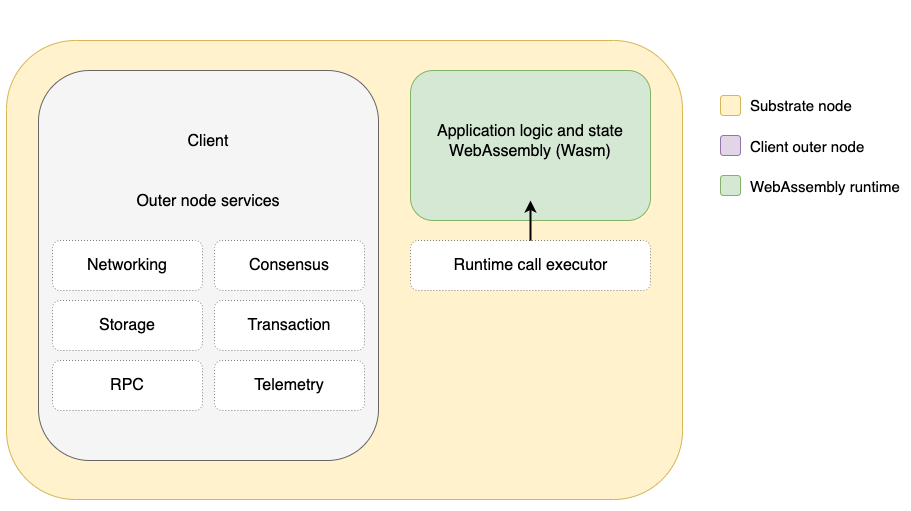
\includegraphics[width=0.8\textwidth]{images/simplified-architecture.png}
  \caption{架构简图}\label{架构简图} % label 用来在文中索引
\end{figure}

高层次概括地说,Substrate节点提供了一个层次化的环境,其中包含两个主要的元素:

\begin{itemize}
\item
  一个带有\textbf{外部节点服务}(outer node
  services)的\textbf{客户端},用于处理网络活动,如发现对等节点、管理交易请求、与对等节点达成共识以及响应RPC调用。
\item
  一个包含了执行区块链的状态转换函数的所有业务逻辑的\textbf{运行时}。
\end{itemize}

\hypertarget{ux5916ux90e8ux8282ux70b9}{%
\textbf{外部节点}\label{ux5916ux90e8ux8282ux70b9}}

外部节点负责运行时外部发生的活动。例如,外部节点负责发现对等节点、管理交易池、与其他节点通信以达成共识,以及响应来自``外部世界''的RPC调用或浏览器请求。

外层节点处理的一些最重要的活动包括以下几种:

\begin{itemize}
\item
  \href{/fundamentals/state-transitions-and-storage/}{存储}:
  使用简单高效的键值对存储层,保存Substrate区块链不断变化的状态。
\item
  \href{/fundamentals/node-and-network-types/}{点对点网络}:
  使用\href{https://libp2p.io/}{libp2p` network
  stack}的Rust实现与其他的网络参与者通信。
\item
  \href{/fundamentals/consensus/}{共识}:
  与其他网络参与者通信,以确保他们对区块链的状态达成共识。
\item
  \href{/build/remote-procedure-calls/}{Remote procedure call(RPC)
  API}: 接收入站的HTTP和WebSocket请求,以便区块链用户与网络交互。
\item
  \href{/maintain/monitor/}{维护节点度量}:
  通过内嵌的\href{https://prometheus.io/}{Prometheus}服务器收集并提供节点度量相关的信息。
\item
  \href{/build/build-process/}{执行环境}:
  为运行时选择要使用的执行环境(WebAssembly或本地的Rust)然后将调用分派给所选的环境。
\end{itemize}

执行这些任务通常需要外部节点查询运行时以获取信息或向运行时提供信息。这种通信通过调用专门的\href{/reference/runtime-apis/}{runtime
APIs}来处理。

\hypertarget{ux8fd0ux884cux65f6}{%
\textbf{运行时}\label{ux8fd0ux884cux65f6}}

运行时确定交易是否有效,并负责处理区块链的状态转换函数的更改。因为运行时能执行它接收到的函数,所以它可以控制如何将交易包含在区块中,以及如何将区块返回到外部节点以传播或导入到其他节点。从本质上讲,运行时负责处理区块链上发生的所有事情,它也是构建Substrate区块链节点的核心组件。

Substrate运行时被设计成编译为\href{/reference/glossary\#webassembly-wasm}{WebAssembly
(Wasm)}字节码的形式。这样的设计决策有如下益处:

\begin{itemize}
\item
  支持无分叉的升级。
\item
  多平台适配。
\item
  可以检查运行时有效性。
\item
  已验证可用于中继链共识机制。
\end{itemize}

与外部节点向运行时提供信息的方式类似,运行时使用专门的\href{https://paritytech.github.io/substrate/master/sp_io/index.html}{主机函数(host
function)}与外部节点或外部世界通信。

\hypertarget{ux8f7bux91cfux7ea7lightuxff09ux5ba2ux6237ux7aefux8282ux70b9}{%
\subsubsection{轻量级(light)客户端节点}\label{ux8f7bux91cfux7ea7lightuxff09ux5ba2ux6237ux7aefux8282ux70b9}}

轻量级客户端或轻量级节点是Substrate节点的简化版本,仅提供运行时和当前状态。它允许用户使用浏览器、浏览器扩展、移动设备或家用电脑直接连接到Substrate运行时。

有了轻量级客户端节点,您就可以使用用Rust、JavaScript或其他语言编写的RPC端口(endpoint)连接到WebAssembly执行环境,以读取区块头(block
header)、提交交易并查看其的结果。

\hypertarget{ux4e0bux4e00ux6b65ux5b66ux4ec0ux4e48}{%
\subsubsection{下一步学什么?}\label{ux4e0bux4e00ux6b65ux5b66ux4ec0ux4e48}}

在您已经对Substrate体系结构和核心节点组件有了基本的认知后,我们建议参阅以下主题以了解更多信息:

\begin{itemize}
\item
  \href{/fundamentals/node-and-network-types}{网络和区块链}
\item
  \href{/fundamentals/transaction-types}{交易和区块基础}
\item
  \href{/fundamentals/transaction-lifecycle/}{交易生命周期}
\item
  \href{/fundamentals/state-transitions-and-storage/}{状态转变和存储}
\item
  \href{/reference/runtime-apis/}{Runtime APIs}
\end{itemize}

\subsection{网络与区块链}

在考虑构建区块链时,我们必须要认识到:定义一个网络离不开边界(boundaries)这一概念。例如,连接到单个路由器的一组计算机可以被认为是一个家庭网络,而防火墙可能是企业网络的边界。通过公共通信协议,较小的孤立网络也可以连接到更大型的网络。

类似地,我们可以认为,区块链网络乃是由其边界,和与其他区块链的关系(孤立、或有所通信)定义的。

作为区块链工程师的工具包,Substrate能够用于开发您能想到的任何类型的区块链,并根据特定于应用程序的需求定义其边界。考虑到这种灵活性,您需要决定您想要构建的网络类型是什么,以及不同节点在该网络中可能扮演的角色。

\hypertarget{ux7f51ux7edcux7c7bux578b}{%
\subsubsection{网络类型}\label{ux7f51ux7edcux7c7bux578b}}

基于Substrate的区块链可用于不同类型的网络架构,例如下列的数种:

\begin{itemize}
\item
  \textbf{私有网络} 仅能访问受限的数个节点的网络。
\item
  \textbf{单链网络}
  拥有各自的安全协议实现,并不与其他区块链网络通信。比特币和以太坊就是这样的网络,不过他们不基于Substrate开发。
\item
  \textbf{中继链(Relay chains)网络}
  为连接到它们的其他网络提供去中心化的安全保障和通信机制。
\item
  \textbf{平行多链(Parachains)网络}
  为连接到中继链而生,也能与使用同一个中继链的其他网络通信。因为平行多链依赖中继链来封装产生的区块,所以平行多链必须使用与它们的目标中继链相同的共识协议。
\end{itemize}

\hypertarget{ux8282ux70b9ux7c7bux578b}{%
\subsubsection{节点类型}\label{ux8282ux70b9ux7c7bux578b}}

区块链要求网络节点同步,以呈现一致且最新的区块链状态视图。每个同步节点存储区块链的副本,并跟踪收到的交易。然而,保存整个区块链的完整副本需要大量的存储空间和计算量,并且下载从创世块到最新区块的所有区块对于大多数区块链的应用场景来说是不实际的。

为了更容易维护链的安全性和完整性,同时减少想要访问区块链数据的客户端对资源的消耗,有不同类型的节点可以与链交互:

\begin{itemize}
\item
  \protect\hyperlink{}{完全节点(Full nodes)}
\item
  \protect\hyperlink{}{归档节点(Archive nodes)}
\item
  \protect\hyperlink{}{轻量级客户端节点(Light client nodes)}
\end{itemize}

\hypertarget{ux5b8cux5168ux8282ux70b9}{%
\textbf{完全节点}\label{ux5b8cux5168ux8282ux70b9}}

完全节点是区块链网络基础设施的关键部分,也是最常见的节点类型;其负责存储区块链数据,并且一般会参与常见的区块链操作,例如创建和验证区块,接收和验证交易,以及响应用户请求。

\begin{figure}[htbp]
  \centering
  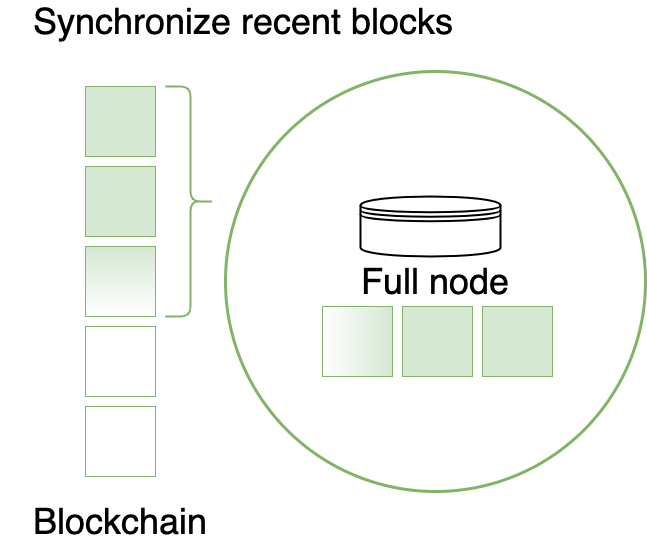
\includegraphics[width=0.6\textwidth]{images/full-node.png}
  \caption{完全节点示意图}\label{完全节点示意图} % label 用来在文中索引
\end{figure}

默认情况下,完全节点被配置为只存储最近的256个块,并丢弃比这更早的状态(创世块除外),以防止全节点无限增长进而消耗所有的磁盘空间。不过,我们也可以配置完全节点保留的区块数量。

虽然较久远的区块被丢弃了,但完全节点会保留从创世块到最近区块的所有\href{/reference/glossary/\#header}{块报头},以对状态的正确性进行验证。完全节点可以访问所有的块标头,所以可以通过执行从创世块开始的所有块(executing
all of the blocks from the genesis
block)来重建整个区块链的状态。检索有关过往状态的信息需要很大的计算量,故通常应该使用存档以代替上述过程。

完完全节点允许您读取链的当前状态,并直接在网络上提交和验证交易。由于丢弃了久远区块中的状态,完整节点所需的磁盘空间比归档节点少得多。不过,一个完全节点需要更多的计算资源来查询和检索关于某些先前状态的信息。如果需要查询历史区块,应该清空这个完全节点,然后将其作为存档节点重新启动。

\hypertarget{ux5f52ux6863ux8282ux70b9}{%
\textbf{归档节点}\label{ux5f52ux6863ux8282ux70b9}}

归档节点类似于完全节点,不过它们会存储所有过去的区块,每个区块都存储有完整的状态信息。这种节点往往在需要访问历史信息的场景下使用(如块浏览器、钱包、论坛和类似的应用程序)。

\begin{figure}[htbp]
  \centering
  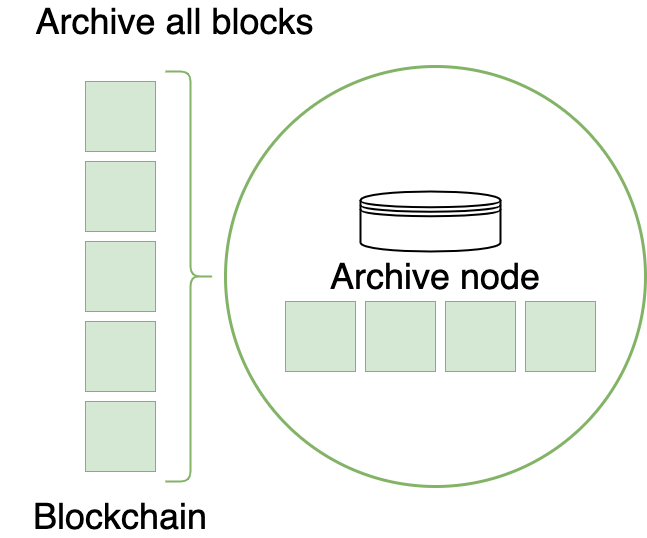
\includegraphics[width=0.6\textwidth]{images/archive-node.png}
  \caption{归档节点示意图}\label{归档节点示意图} % label 用来在文中索引
\end{figure}

由于归档节点保存着历史状态,它们将消耗大量磁盘空间,这也是它们不如完全节点常见的原因。不过,归档节点可以方便地查询区块链在任何时间点的过去状,例如查找某个区块中的帐户余额,或者查看导致指定状态更改的交易的详细信息。当在归档节点存储的数据上运行这些类型的查询时,它们会更快、更高效。

\hypertarget{ux8f7bux91cfux7ea7ux5ba2ux6237ux7aefux8282ux70b9}{%
\textbf{轻量级客户端节点}\label{ux8f7bux91cfux7ea7ux5ba2ux6237ux7aefux8282ux70b9}}

轻量级客户端节点使您能够以最低的硬件要求连接到Substrate网络。

\begin{figure}[htbp]
  \centering
  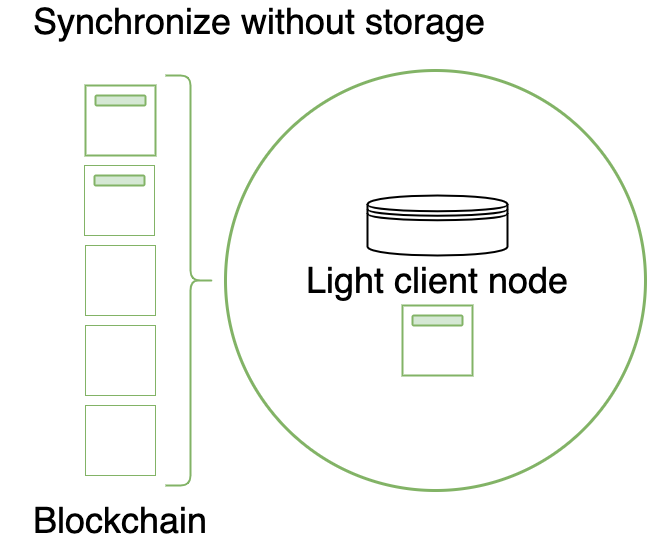
\includegraphics[width=0.6\textwidth]{images/light-node.png}
  \caption{轻节点示意图}\label{轻节点示意图} % label 用来在文中索引
\end{figure}

因为轻量级客户端节点需要的系统资源最少,所以它们可以嵌入到基于web的应用程序、浏览器扩展、移动设备应用程序或物联网(IoT)设备中。这类节点通过RPC端口提供运行时和对当前链状态的访问。轻量级客户端节点的RPC端口可以用Rust、JavaScript或其他语言编写,用于读取区块头、提交交易和查看其结果。

轻量级客户端节点不参与区块链和网络操作。例如,轻客户端节点不负责产生或验证区块,也不会传播交易或达成共识。它们也不会存储任何过去的块,因此如果不向拥有历史数据的节点请求,它就无法读取历史数据。

\hypertarget{ux8282ux70b9ux89c4ux5219node-rolesuxff09}{%
\subsubsection{节点规则(Node
roles)}\label{ux8282ux70b9ux89c4ux5219node-rolesuxff09}}

根据启动节点时指定的命令行选项,节点可以在区块链的运行过程中扮演不同的角色,并可以提供对链上状态的不同级别的访问。例如,您可以指定哪些节点有权生产新区块,哪些节点可以与对等节点通信。未被授权生产区块的对等节点可以导入(import)新区块,接收交易,并向其他节点发送和接收有关新交易的消息(gossip)。除此之外,您还可以阻止节点连接到更广泛的网络,并限制节点与特定节点通信。

\hypertarget{ux4e0bux4e00ux6b65ux5b66ux4ec0ux4e48}{%
\subsubsection{下一步学什么?}\label{ux4e0bux4e00ux6b65ux5b66ux4ec0ux4e48}}

您可以使用Substrate构建几乎任何类型的网络------从完全自包含的私有单链到您自己的中继链生态系统或兼容的平行副链。

请参阅以下页面,以更深入地研究网络和节点类型:

\begin{itemize}
\item
  \href{/tutorials/get-started/build-local-blockchain/}{构建本地链}
\item
  \href{/tutorials/get-started/simulate-network/}{模拟网络}
\item
  \href{/tutorials/get-started/add-trusted-nodes/}{添加可信节点}
\item
  \href{/tutorials/get-started/authorize-specific-nodes/}{认证指定节点}
\end{itemize}
